%%%%%%%%%%%%%%%%%%%%%%%%%%%%%%%%%%%%%%%%%
% Short Sectioned Assignment
% LaTeX Template
% Version 1.0 (5/5/12)
%
% This template has been downloaded from:
% http://www.LaTeXTemplates.com
%
% Original author:
% Frits Wenneker (http://www.howtotex.com)
%
% License:
% CC BY-NC-SA 3.0 (http://creativecommons.org/licenses/by-nc-sa/3.0/)
%
%%%%%%%%%%%%%%%%%%%%%%%%%%%%%%%%%%%%%%%%%

%----------------------------------------------------------------------------------------
%	PACKAGES AND OTHER DOCUMENT CONFIGURATIONS
%----------------------------------------------------------------------------------------

\documentclass[paper=a4, fontsize=11pt]{scrartcl} % A4 paper and 11pt font size

\usepackage{graphicx}
\usepackage[T1]{fontenc} % Use 8-bit encoding that has 256 glyphs
\usepackage{fourier} % Use the Adobe Utopia font for the document - comment this line to return to the LaTeX default
\usepackage[english]{babel} % English language/hyphenation
\usepackage{amsmath,amsfonts,amsthm} % Math packages

\usepackage{lipsum} % Used for inserting dummy 'Lorem ipsum' text into the template
\usepackage{algorithm}
\usepackage{algpseudocode}
\usepackage{sectsty} % Allows customizing section commands
\allsectionsfont{\scshape} % Make all sections centered, the default font and small caps

\usepackage{algorithm,algpseudocode}% http://ctan.org/pkg/{algorithms,algorithmx}
\algnewcommand{\Inputs}[1]{%
  \State \textbf{Inputs:}
  \Statex \hspace*{\algorithmicindent}\parbox[t]{.8\linewidth}{\raggedright #1}
}
\algnewcommand{\Initialize}[1]{%
  \State \textbf{Initialize:}
  \Statex \hspace*{\algorithmicindent}\parbox[t]{.8\linewidth}{\raggedright #1}
}

\usepackage{fancyhdr} % Custom headers and footers
\pagestyle{fancyplain} % Makes all pages in the document conform to the custom headers and footers
\fancyhead{} % No page header - if you want one, create it in the same way as the footers below
\fancyfoot[L]{} % Empty left footer
\fancyfoot[C]{} % Empty center footer
\fancyfoot[R]{\thepage} % Page numbering for right footer
\renewcommand{\headrulewidth}{0pt} % Remove header underlines
\renewcommand{\footrulewidth}{0pt} % Remove footer underlines
\setlength{\headheight}{13.6pt} % Customize the height of the header

\numberwithin{equation}{section} % Number equations within sections (i.e. 1.1, 1.2, 2.1, 2.2 instead of 1, 2, 3, 4)
\numberwithin{figure}{section} % Number figures within sections (i.e. 1.1, 1.2, 2.1, 2.2 instead of 1, 2, 3, 4)
\numberwithin{table}{section} % Number tables within sections (i.e. 1.1, 1.2, 2.1, 2.2 instead of 1, 2, 3, 4)

\setlength\parindent{0pt} % Removes all indentation from paragraphs - comment this line for an assignment with lots of text

%----------------------------------------------------------------------------------------
%	TITLE SECTION
%----------------------------------------------------------------------------------------

\newcommand{\horrule}[1]{\rule{\linewidth}{#1}} % Create horizontal rule command with 1 argument of height

\title{	
\normalfont \normalsize
\textsc{Rice University, Department of Computer Science} \\ [25pt] % Your university, school and/or department name(s)
\horrule{0.5pt} \\[0.4cm] % Thin top horizontal rule
\huge Assignment 0, COMP 576 \\ % The assignment title
\horrule{2pt} \\[0.5cm] % Thick bottom horizontal rule
}

\author{Yuanyuan Zhu(yz281)} % Your name

\date{\normalsize\today} % Today's date or a custom date

\begin{document}

\maketitle % Print the title

%----------------------------------------------------------------------------------------
%	PROBLEM 1
%----------------------------------------------------------------------------------------

\section{Task 1}
\begin{verbatim}
(groq) YuanyuanZhu@Yuanyuan-MBP hw2problem4 % conda info
/opt/anaconda3/lib/python3.12/site-packages/conda/base/context.py:198: FutureWarning: Adding 'defaults' to channel list implicitly is deprecated and will be removed in 25.9. 

To remove this warning, please choose a default channel explicitly with conda's regular configuration system, e.g. by adding 'defaults' to the list of channels:

  conda config --add channels defaults

For more information see https://docs.conda.io/projects/conda/en/stable/user-guide/configuration/use-condarc.html

  deprecated.topic(

     active environment : groq
    active env location : /opt/anaconda3/envs/groq
            shell level : 2
       user config file : /Users/YuanyuanZhu/.condarc
 populated config files : /Users/YuanyuanZhu/.condarc
          conda version : 25.3.0
    conda-build version : 24.5.1
         python version : 3.12.2.final.0
                 solver : classic
       virtual packages : __archspec=1=m1
                          __conda=25.3.0=0
                          __osx=12.5.1=0
                          __unix=0=0
       base environment : /opt/anaconda3  (writable)
      conda av data dir : /opt/anaconda3/etc/conda
  conda av metadata url : None
           channel URLs : https://repo.anaconda.com/pkgs/main/osx-arm64
                          https://repo.anaconda.com/pkgs/main/noarch
                          https://repo.anaconda.com/pkgs/r/osx-arm64
                          https://repo.anaconda.com/pkgs/r/noarch
          package cache : /opt/anaconda3/pkgs
                          /Users/YuanyuanZhu/.conda/pkgs
       envs directories : /opt/anaconda3/envs
                          /Users/YuanyuanZhu/.conda/envs
               platform : osx-arm64
             user-agent : conda/25.3.0 requests/2.32.3 CPython/3.12.2 Darwin/21.6.0 OSX/12.5.1 aau/0.4.4 c/OR1hgsDochgv8vl6J1XGxQ s/rIjiG9fnGbbxUGUrfL8gcA e/nAiaYCw9yHTNnUIxvY56gA
                UID:GID : 501:20
             netrc file : None
           offline mode : False
\end{verbatim}

\section{Task 2}
N/A

\section{Task 3}
\begin{verbatim}
import matplotlib.pyplot as plt
plt.plot([1,2,3,4], [1,2,7,14], 'ro')
plt.axis([0, 6, 0, 20])
plt.show()
\end{verbatim}
\begin{figure}[H]
 	\centering
 	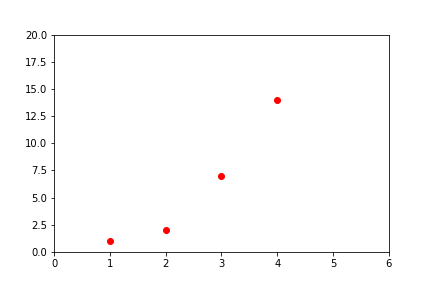
\includegraphics[scale=0.75]{./../foo1.png}
 	\caption{exported figure of matplotlib}
 	\label{fig:matplotlib_output}
\end{figure}

\section{Task 4}
\begin{verbatim}
import numpy as np
import matplotlib.pyplot as plt
ax = plt.subplot(111)
t = np.arange(0.0, 10.0, 0.01)
s = np.cos(2*np.pi*t)+1
line, = plt.plot(t, s, lw=2)
plt.ylim(-1,3)
plt.savefig('foo2.png')
plt.show()
\end{verbatim}
\begin{figure}[H]
 	\centering
 	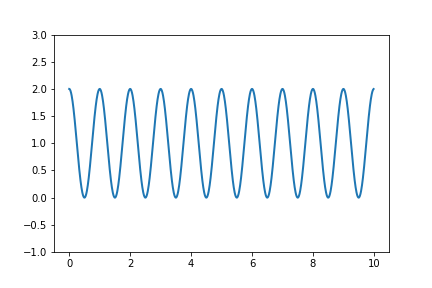
\includegraphics[scale=0.75]{./../foo2.png}
 	\caption{exported figure of matplotlib}
 	\label{fig:matplotlib_output}
\end{figure}

\section{Task 5}
Github Account: YuanyuanZ0908

\section{Task 6}
https://github.com/YuanyuanZ0908/COMP576

\end{document}

